\lecture{2}{Бор. Алгоритм Ахо-Корасик.}
\subsection{Структура данных бор.}
Рассмотрим дерево, в котором каждому ребру соответствует некоторый символ.
Тогда мы можем интерпретировать символы на ребрах на пути из корня в вершину как символы некоторой строки.
Мы получили \highlight{бор}, или же, более формально:

\begin{definition}
        \highlight{Бор} --- структура данных для хранения строк, которая представляет из себя 
        подвешенное дерево с символами на рёбрах и удовлетворяет некоторым свойствам.
\end{definition}

Основные свойства бора:
\begin{itemize}
        \item Нет ребёр с одинаковыми символами, выходящих из одной вершины.
        \item Вершины, которые являются последними в некоторой строке, помечаются как терминальные. 
\end{itemize}

\begin{figure}[htbp]
        \caption*{Пример бора.}
        \begin{center}
                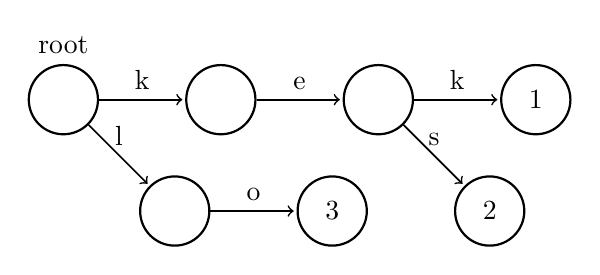
\begin{tikzpicture}[
                        -> = stealth,
                        shorten > = 1pt,
                        auto,
                        node distance = 2cm,
                        semithick
                        ]

                        \tikzstyle{point}=[
                                draw = black,
                                circle,
                                thick,
                                fill = white,
                                minimum size = 25pt
                        ]

                        \node[point] (1) [label=above: root] {};
                        \node[point] (2) [right of=1] {};
                        \node[point] (3) [right of=2] {};
                        \node[point] (4) [right of=3]  {1};
                        \node[point] (5) [below right of=3] {2};
                        \node[point] (6) [below right of=1] {};
                        \node[point] (7) [right of=6] {3};
                        
                
                        \draw (1) -- (2) node[midway, above] {k}; 
                        \draw (2) -- (3) node[midway, above] {e}; 
                        \draw (3) -- (4) node[midway, above] {k}; 
                        \draw (3) -- (5) node[midway, above] {s}; 
                        \draw (1) -- (6) node[midway, above] {l}; 
                        \draw (6) -- (7) node[midway, above] {o}; 
                \end{tikzpicture}
        \end{center}
\end{figure}

В примере выше массив строк следующий:  \textit{kek, kes, lo}.

Теперь давайте разберёмся, как строить бор. Будем хранить в каждой вершине информацию о том, является ли
она листом (т.е. существует ли строка, которая оканчивается на вершине) и массив указателей на детей вершин
\texttt{next}, где \texttt{next[i]} --- указатель на вершину, в которую ведёт ребро с индексом
\texttt{i}.

Теперь для построения бора встанем в корень и посмотрим, есть ли из неё переход по ребру \texttt{s[i]}
(\texttt{s} --- строка, которую мы вставляем в бор), так проходим по всем символам строки и ставим
метку на вершине, в которую дошли.

\begin{remark}
  Вставка в \textbf{бор} происходит за $O(n)$, а потребляемая память --- $O(nk)$, где  $k$ --- размер алфавита.
\end{remark}

\subsection{Алгоритм Ахо-Корасик.}

Пусть у нас есть набор строк-образцов \texttt{pattern[i]} и некоторая строка \texttt{s},
необходимо эффективно искать всех вхождения образцов в текст. Для этой задачи воспользуемся алгоритмом
\textbf{Ахо-Корасик.}

\begin{enumerate}
  \item Строим \textbf{бор} из входных строк за $O(m)$, где  $m$---длина строк.
        \item Создание суффиксных ссылок.

        Это who? Для их осознания представим ситуацию, что мы, как обычно, гуляли по бору, но тут вдруг
        оказалось, что идти нам некуда (вот блин). Тогда, с одной стороны, мы можем пойти в корень и 
        отправиться гулять дальше, но вдруг какой-то паттерн начинается также, как и суффикс того, по чему 
        мы прошли. Например, у нас набор строк состоит из $abcd$ и  $bca$, и
        вот мы гуляем по строке $abca$. Мы пришли по рёбрам  $a, b, c$ бора и оказывается, что есть только
        один путь (не путю) по ребру $d$, а следующий символ в нашей строке $a$, что вместе с пройденными
        ранее $bc$ образуют один из наших паттернов. Т.е. нам нужно научиться как-то быстро переходить 
        к наибольшему собственному суффиксу пройденного пути в случае неудачи. На помощь приходят
        суффиксные ссылки! Теперь более формально.
        \begin{definition}
                \highlight{Суффиксная ссылка} --- это вершина, в которой оканчивается наидлиннейший
                собственный суффикс. Суффиксная ссылка корня для удобства будет ссылкой на корень.
        \end{definition}
       Теперь пока в текущей вершине нет перехода по соответствующей букве, мы выполняем переход по
       суффиксной ссылке. Таким образом мы вводим важное понятие \highlight{функции перехода} из вершины $v$ 
       по символу $c$, которая определяется следующим образом:
       \begin{itemize}
                \item корень бора, если текущая вершина --- корень. 
                \item \texttt{v.next[c]}, где \texttt{next} --- массив переходов из текущей вершины, если
                переход \texttt{c} существует.
                \item \texttt{v.child[c]}, где \texttt{child} --- массив детей из текущей вершины,
                если ребёнок по ребру \texttt{c} существует.
                \item функция перехода по символу $c$ от вершины по суффиксной ссылке.
       \end{itemize}
       
       Теперь научимся искать суффиксные ссылки. Заметим, что нам достаточно пройти в родителя вершины
       (пусть мы сделали это по ребру $c$), пройти
       по его суффиксной ссылке и выполнить переход (т.е. функцию перехода) по ребру $c$. 
       Интересно, что функцию перехода мы определили с использованием суффиксных ссылок, а
       суффиксные ссылки --- с помощью функции перехода. Мы получили двойную рекурсию.
       Рассмотрим подробнее на примере.

       \begin{figure}[H]
               \caption*{Пример нахождения суффиксной ссылки}
               \begin{center}
                       \begin{tikzpicture}[    
                                -> = stealth,    
                                shorten > = 1pt,    
                                auto,    
                                node distance = 3cm,    
                                semithick    
                                ]    
                                
                                \tikzstyle{point}=[    
                                        draw = black,    
                                        circle,    
                                        thick,    
                                        fill = white,    
                                        minimum size = 25pt    
                                ]    
                                
                                \node[point] (1) [] {root};    
                                \node[point] (2) [right of=1] {};
                                \node[point] (3) [right of=2] {p};
                                \node[point] (4) [right of=3] {v};
                                \node[point] (5) [below right of=1] {};
                                \node[point] (6) [right of=5] {g};
                                \node[point] (7) [right of=6] {2};
                              

                                \draw (1) -- (2) node [midway, above] {a};
                                \draw (2) -- (3) node [midway, above] {b};
                                \draw (3) -- (4) node [midway, above] {c};
                                \draw (1) -- (5) node [midway, above] {b};
                                \draw (5) -- (6) node [midway, above] {c};
                                \draw (6) -- (7) node [midway, above] {d};
                                \draw (3) -- (5) node [midway, right] {суфф.};
                       \end{tikzpicture}
               \end{center}
       \end{figure}
       Пусть у нас есть такой бор и уже есть суффиксная ссылка для вершины $p$.
       Теперь найдём суффиксную ссылку для вершины $v$. Пойдём в родителя $p$ и перейдём по его суффиксной
       ссылке. Мы получили возможный максимальный собственный суффикс для нашей вершины $v$, осталось
       выполнить переход по символу $c$, в данном случае мы попадём в следующую вершину $g$, но могли
       перейти по следующей суффиксной ссылке и ещё уменьшить наш суффикс. Итого:
       \begin{figure}[H]
               \caption*{Пример нахождения суффиксной ссылки}
               \begin{center}
                       \begin{tikzpicture}[    
                                -> = stealth,    
                                shorten > = 1pt,    
                                auto,    
                                node distance = 3cm,    
                                semithick    
                                ]    
                                
                                \tikzstyle{point}=[    
                                        draw = black,    
                                        circle,    
                                        thick,    
                                        fill = white,    
                                        minimum size = 25pt    
                                ]    
                                
                                \node[point] (1) [] {root};    
                                \node[point] (2) [right of=1] {};
                                \node[point] (3) [right of=2] {p};
                                \node[point] (4) [right of=3] {v};
                                \node[point] (5) [below right of=1] {};
                                \node[point] (6) [right of=5] {g};
                                \node[point] (7) [right of=6] {2};
                              

                                \draw (1) -- (2) node [midway, above] {a};
                                \draw (2) -- (3) node [midway, above] {b};
                                \draw (3) -- (4) node [midway, above] {c};
                                \draw (1) -- (5) node [midway, above] {b};
                                \draw (5) -- (6) node [midway, above] {c};
                                \draw (6) -- (7) node [midway, above] {d};
                                \draw (3) -- (5) node [midway, right] {суфф.};
                                \draw (4) -- (6) node [midway, right] {суфф.};
                       \end{tikzpicture}
               \end{center}
       \end{figure}
       Таким образом суффиксные ссылки и функцию перехода можно вычислять ленивой динамикой.
       Достаточно сохранять уже посчитанные значения функции перехода и суффиксных ссылок.
       \item Создание сжатых суффиксных ссылок.

        Возможна ситуация, когда суффиксных ссылок становится слишком много. Например, если наш бор
        выродился в <<бамбук>> без ветвления. Тогда нам дорого хранить массив всех шаблонов, которые
        оканчиваются в вершине. Решением большого количества переходов по суффиксным ссылкам и излишнего
        хранения могут стать сжатые суффиксные ссылки.
        \begin{definition}
                \highlight{Сжатая суффиксная ссылка} --- такая ссылка, которая образована несколькими
                переходами по обычным суффиксным ссылкам, и ведёт сразу в терминальную вершину.
        \end{definition}
        Тогда решением проблемы хранение будет обход по сжатым суффиксным ссылкам. 
        Также с помощью сжатых суффиксных ссылок решается задача о поиске всех строк из
        заданного набора в тексте.
\end{enumerate}

\subsection{Оценка времени работы алгоритма Ахо-Корасик.}
Пусть $n$ --- количество вершин, $m$ --- суммарная длина паттернов, $k$ --- количество ответов.

Тогда обработка одного символа текста складывается из:
\begin{itemize}
        \item Построение бора по паттернам за $O(m)$.
        \item Вызов функции перехода. Ленивое построение для каждого узла и символа вычисляет функцию
        не более раза. Итого: $O(n + m)$.
        \item Построение суффиксных ссылок по одному вызову на каждую вершину бора.
        Каждый переход по сжатой ссылке либо находит ответ, либо приходит в корень.
\end{itemize}
Итого получаем: $O(n + m + k)$.
